\section{Einleitung und Versuchsziel}
\label{sec:aufgabenstellung}
%- Darstellung des Versuchsziels und der in dem Versuch bearbeiteten Fragestellungen.
%- Kurze Einführung grundlegenden theoretischen Zusammenhänge und der
%Gleichungen die für den Versuch und die Versuchsauswertung relevant sind.
%- Alle Abbildungen sind durchzunummerieren (Abb. 01, …) und mit einer Bild- bzw.
%Tabellenunterschrift zu versehen. Externe Quellen sind in der Bildunterschrift als
%Literatur-Nummer (Quelle: [1]) oder Literatur-Kürzel (Quelle: [Schmidt2015])
%anzugeben.Physikalische Chemie
%FB Ingenieur- und Naturwissenschaften
%Protokollvorlage PC-II Praktikum, SoSe 2020 2
%- Alle Formeln sind durchzunummerieren.
%- Benennung der experimentellen Geräte und Hilfsmittel mit denen der Versuch
%durchgeführt wird (Bsp: Thermostat Firma/Typ XY, Druckmessröhre Firma/Typ Z).

Im Praktikumsversuch "`Oberflächenspannung an Grenzflächen"' werden verschiedene, wässrige Proben auf ihre Oberflächenspannung untersucht. Zudem ist die Temperaturabhängigkeit der Oberflächenspannung mit Hilfe von Wasser zu analysieren.\\
Die Vorgänge an Grenzflächen  sind von großer Bedeutung für Prozesse mit Phasenwechsel. Um diese charakterisieren und weitere rechnerische Vorhersagen treffen zu können, ist die Oberflächenspannung ein entscheidender Bestandteil für diese Beschreibungen.

\section*{Theoretische Grundlagen}
\subsection*{Kohäsions- und Adhäsionskräfte}
Zwischen Teilchen in einer flüssigen Phasen herrschen Wechselwirkungskräfte. Diese sind bedingt durch Anziehungskräfte der Teilchen untereinander in der Flüssigkeit. Für homogen verteilte Teilchen innerhalb der flüssigen Phase resultiert, aufgrund der geringen Reichweite dieser Kräfte, eine Gesamtkraft von null. Betrachtet man die Teilchen, welche sich direkt an der Phasengrenze der Flüssigkeit befinden, so ist dieser zuvor beschriebene Zusammenhang ungültig. Da auf diese Grenzteilchen, auch \textsc{Bulk}-Teilchen genannt, auch Kräfte aus der benachbarten Phase und nicht nur aus der eigenen Phase wirken, können hier resultierende Kräfte größer  oder kleiner null sein. Diese resultierende Kraft steht in diesem Fall senkrecht zur Grenzfläche.\linebreak
Im Folgenden wird für die Beschreibung von Kräften innerhalb der stoffeigenen Phase von Kohäsions- und Kräften zwischen Phasen von Adhäsionskräften gesprochen. Sind die Adhäsionskräfte signifikant größer als die Kohäsionskräfte so maximiert die betrachtete Flüssigkeit ihre Oberfläche der Grenzschicht. Die resultierende Kraft wirkt hierbei entgegensetzt zum Phaseninneren der Flüssigkeit. Wirkt die resultierende Kraft in das Phaseninnere so sind die Kohäsionskräfte größer als die Adhäsionskräfte und die Grenzfläche der Flüssigkeit ist versucht ihre Oberfläche zu minimieren.

\subsection*{Ringmethode nach \textsc{Du Noüy}}
Die Abreißmethode nach \textsc{Du Noüy} wird zur Bestimmung von Oberflächenspannungen von $v$-$l$- sowie $l$-$l$-Systemen genutzt. Bei dieser Methode wird mittels Torsionswaage  die wirkende Kraft beim langsamen Herausziehen eines Platin-Iridium-Ringes, welcher in die Flüssigkeit eingetaucht wird. Die wirkende Kraft am Ring wird nun solang erhöht bis die Benetzung der Flüssigkeit abreißt. Die letzte maximal wirkende Kraft entspricht dann der Oberflächenspannung.
\newpage
Das angehobene Flüssigkeitsvolumen durch Ring und Torsionswaage wirkt dabei der angelegten Kraft am Ring entgegen. Für die Oberflächenspannung ergibt sich dann:
\begin{flalign}
\label{gl:zyl}
	\sigma	&= \frac{F_{\text{max}}}{4*\pi *R_{\text{mittel}}}
\end{flalign}
Zu beachten gilt es, dass für die Gleichung \eqref{gl:zyl} die Annahme getroffen, dass ein idealer Zylinder angehoben wird. In der Realität zeigt sich, jedoch ein gekrümmtes Volumen, welches in die Berechnung mit einbezogen werden muss (siehe Abb. \ref{fig:ring_real}). 
\begin{figure}[h!]
	\centering
	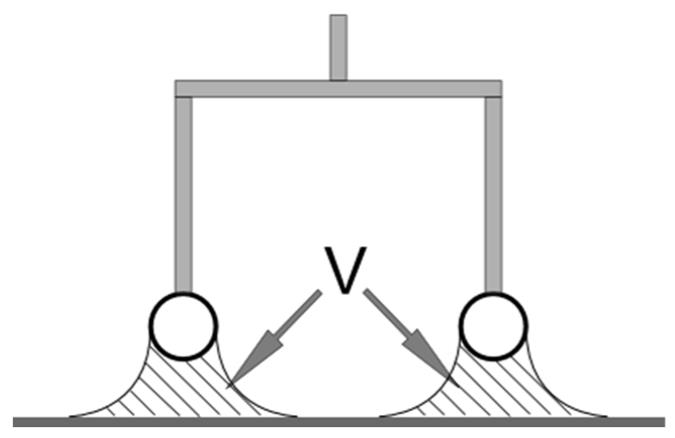
\includegraphics[width=0.5\textwidth]{img/real}
	\caption{Schematische Darstellung des tatsächlich angehobenen Flüssigkeitsvolumens}
	\label{fig:ring_real}
\end{figure}
\FloatBarrier
%Ende
Im Rahmen des Praktikums erfolgt diese Einbeziehung anhand eines Korrekturfaktors. Dafür wird über den Mittelwert der gemessenen Oberflächenspannung, für ein bestimmtes Stoffsystem, einer bestimmten Temperatur $\sigma$ und dem zugehörigen theoretischen Wert der Oberflächenspannung $\sigma^\ast$ ein Verhältnis gebildet. Der Korrekturfaktor $K$.

\begin{flalign}
	K_{kal}&=\frac{\bar{x}}{x_{\text{theor.}}}\\
	K_{kal} &= \frac{\sigma^\ast}{\sigma}
\end{flalign}

\textbf{Mittelwert:}
\begin{flalign}
\label{Gl:Mittelwert}
\bar{x} &= \frac{\sum_{n=1}^{N}x_n}{N}
\end{flalign}

\textbf{Standardabweichung:}
\begin{flalign}\label{Gl:standardabweichung}
s &= \sqrt{\frac{\sum_{n=1}^{N}(x_n-\bar{x})^2}{N-1}}
\end{flalign}

\textbf{relative Standardabweichung:}
\begin{flalign}\label{gl:rel_s}
s_{rel}&=\frac{s}{\bar{x}}
\end{flalign}

\textbf{Ausreißertest:}
\begin{flalign}\label{gl:ausreißero}
\text{obere Grenze} &=\bar{x} + 3*s
\end{flalign}
\begin{flalign}\label{gl:ausreißeru}
\text{untere Grenze} &=\bar{x} - 3*s
\end{flalign}